\documentclass{article}
\usepackage{geometry, graphicx, float, subfigure, amsmath, bm, threeparttable,multirow, multicol, caption}
\usepackage[marginal]{footmisc}
\geometry{a4paper,scale=0.8}
\setlength{\parindent}{2em}
%\captionsetup{font = {small}}

\title{\bf{The Analysis of Probabilities of Conjugation between E.coli and Transposition Mutagenesis of }$kan^R$}
\author{Xun Zhao (Partner: Chase)}
\date{April 19, 2019}

\begin{document}
    \begin{titlepage}
        \maketitle
        \setcounter{page}{0}
        \thispagestyle{empty}
    \end{titlepage}

    \renewcommand{\abstractname}{Introduction}
    \begin{abstract}
		The "jumping" gene was dicovered by McClintock who found spots on corn with different colors. Later, it was found that this phenomenon also happens in other species. 
		
		Conjugation is a cell-to-cell contact that can transfer plasmid and the genes on this plasmid from one bacteria cell to another, through a mating bridge called pilus. Transposon is a part of DNA sequence that can move or duplicate itself from one place to another even to different chromosomes. When the transposon is inserted into a gene, it can knock out the old gene and replace its function with new gene's function, which is called transposition mutagenesis.

		The first part of this experiment is to mate two strains of \emph{E.coli}, and let conjugation happens. The second part is using IPTG to induce $kan^R$ transposon on the plasmid to transpose.

		If conjugation happens, the recipient cell will get the $cm^R$ gene from pVJT128 plasmid, becoming insensitive to chloramphenicol. If transposition happens, the cell will have functional $kan^R$ gene, and become insensitive to kanamycin. If transposition mutagenesis happens at the \emph{lacZ} gene, the colony will be white on X-gel plates, due to it does not have the functional enzyme to digest X-gel.
	\end{abstract}

	\section{Results}
		\subsection{Conjugation}
			\begin{table}[H]
				\caption{Conjugation Data}
				\centering
				\begin{tabular}{|c|c|c|c|c|c|}
					\hline
					Mating Tube&Dilution&$10^0$&$10^{-1}$&$10^{-2}$&$10^{-3}$\\\cline{2-6}
					Cm-Nal Plates&\#Colonies&508&2&0&0\\\hline
					Recipient Tube&Dilution&$10^{-5}$&$10^{-6}$&$10^{-7}$\\\cline{2-5}
					NA Plates&\#Colonies&946&107&13\\\cline{1-5}
					Recipient Tube&Dilution&$10^0$\\\cline{2-3}
					Cm Plates&\#Colonies&135\\\cline{1-3}
					Donor Tube&Dilution&$10^0$\\\cline{2-3}
					Nal Plates&\#Colonies&0\\\cline{1-3}
				\end{tabular}
				\label{conjugation.data}
			\end{table}
		\subsection{Percent Conjugation}
			$$
			\begin{aligned}
			\text{Conjugation}\% &= \frac{\#\text{Cm.Nal} - \#\text{Reversion.Recipient} - \#\text{Reversion.Donor}}{\#\text{NA.Total}}\\
			&= \frac{508 - 135- 0}{\frac{946 + 107 \times 10 + 13 \times 100}{3} \times 10 ^{5}}\\
			&= \frac{373}{1105 \times 10 ^ 5}\times 100\%\\
			&\approx 3.4 \times 10 ^ {-4}\%
			\end{aligned}
			$$
		\subsection{Transposition and Mutagenesis}
			\begin{table}[H]
				\caption{Transposition and Mutagenesis Data}
				\centering
				\begin{tabular}{|c|c|c|c|c|c|c|}
				\hline
				\multirow{3}*{\shortstack{Inducing Tube\\X-gel Kan Plates}}&\multicolumn{2}{|c|}{Dilution}&$10^0$&$10^{-1}$&$10^{-2}$&$10^{-3}$\\\cline{2-7}
				~&\multirow{2}*{\#Colonies}&White&-&3&0&0\\\cline{3-7}
				~&~&Blue&-&8654&728&94\\\hline
				Inducing Tube&\multicolumn{2}{|c|}{Dilution}&$10^{-4}$&$10^{-5}$&$10^{-6}$&$10^{-7}$\\\cline{2-7}
				NA Plates&\multicolumn{2}{|c|}{\#Colonies}&-&820&103&12\\\hline
				\end{tabular}
				\label{transposition.mutagenesis.data}
			\end{table}
		\subsection{Percent Transposition}
			$$
			\begin{aligned}
			\text{Transposition}\% &= \frac{\#\text{X-gel.Kan}}{\#\text{NA.Total}}\\
			&= \frac{((8654 + 3) + 728 \times 10 + 94 \times 100) / 3}{((103 \times 10 + 12 \times 100) / 2) \times 10 ^4}\\
			&= \frac{8445}{1115 \times 10 ^4} \times 100\%\\
			&\approx 0.076\%
			\end{aligned}
			$$
		\subsection{Percent Mutagenesis}
			$$
			\begin{aligned}
			\text{Mutagenesis}\% &= \frac{\#\text{X-gel.Kan.White}}{\#\text{X-gel.Kan.Total}}\\
			&= \frac{3}{((8654 + 3) + 728 \times 10 + 94 \times 100) / 3}\\
			&= \frac{3}{8445} \times 100\%\\
			&\approx 0.35\%
			\end{aligned}
			$$
	\section{Discussion}
		\subsection{Conjugation}
			\begin{figure}[H]
				\begin{minipage}[t]{0.24\textwidth}
					\centering
					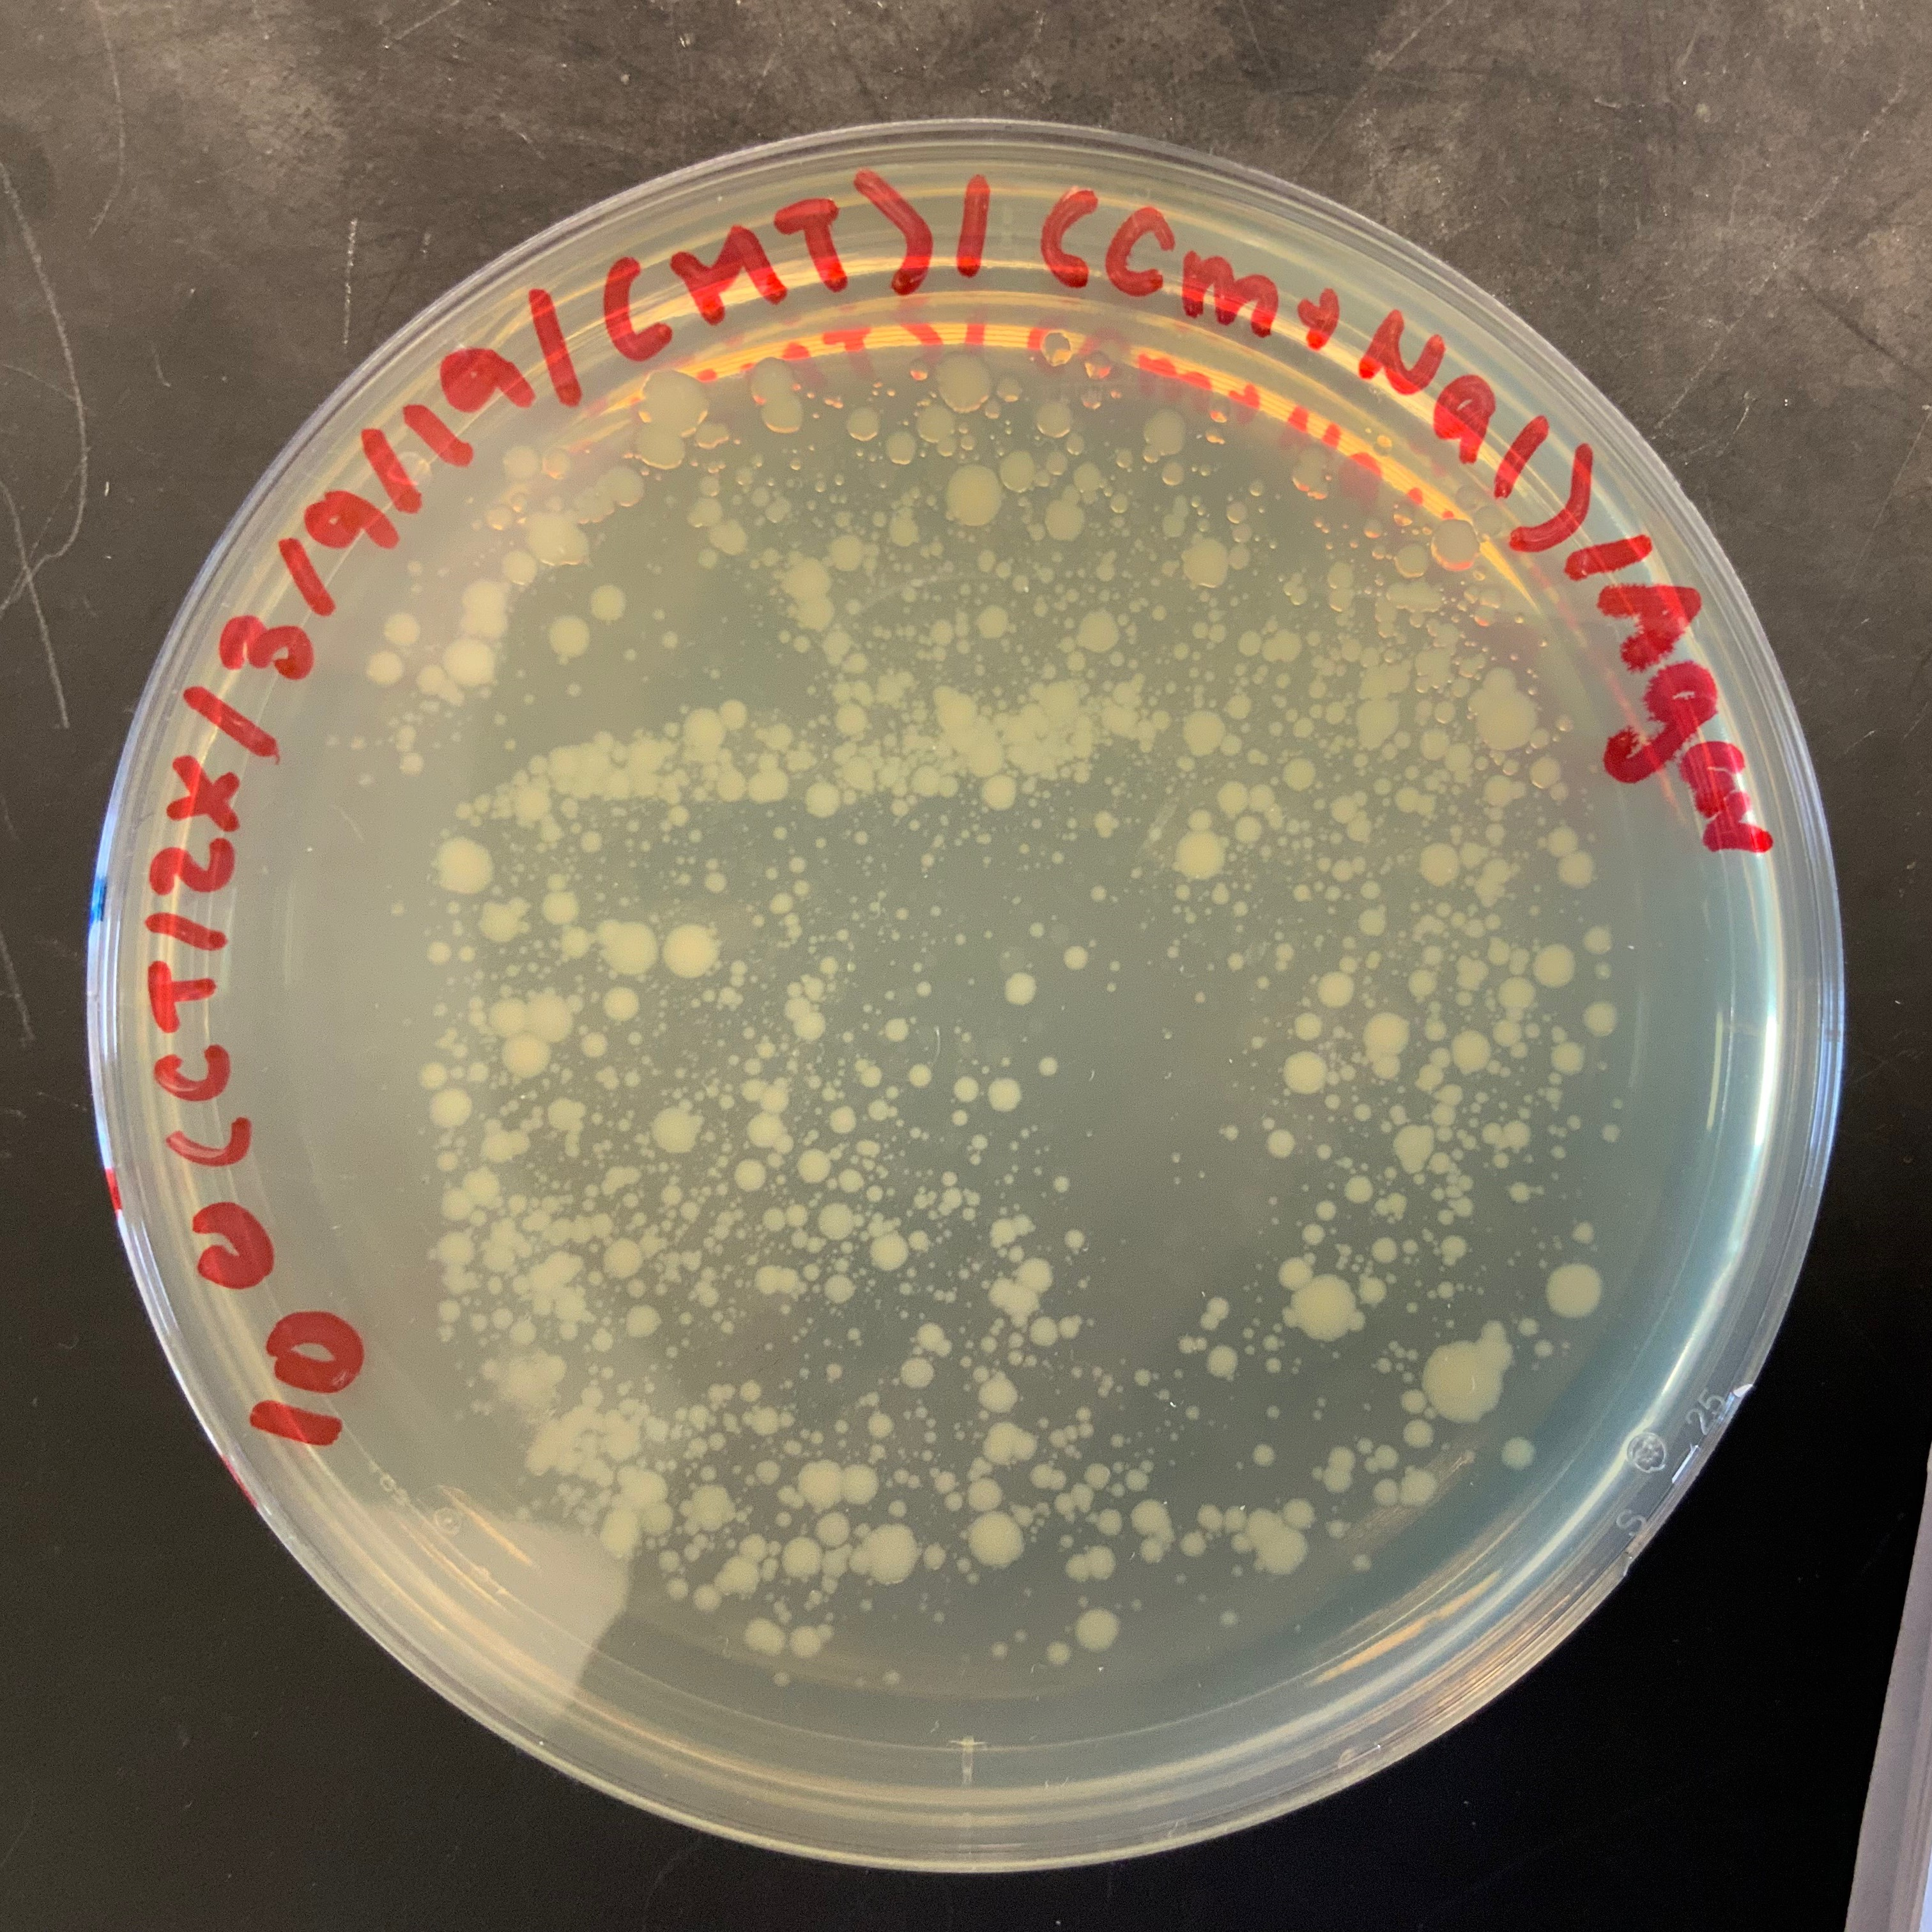
\includegraphics[width = 0.9\linewidth]{Mate_0_NalCm.jpg}
					\caption{MT $10^{0} = 508$}
				\end{minipage}
				\begin{minipage}[t]{0.24\textwidth}
					\centering
					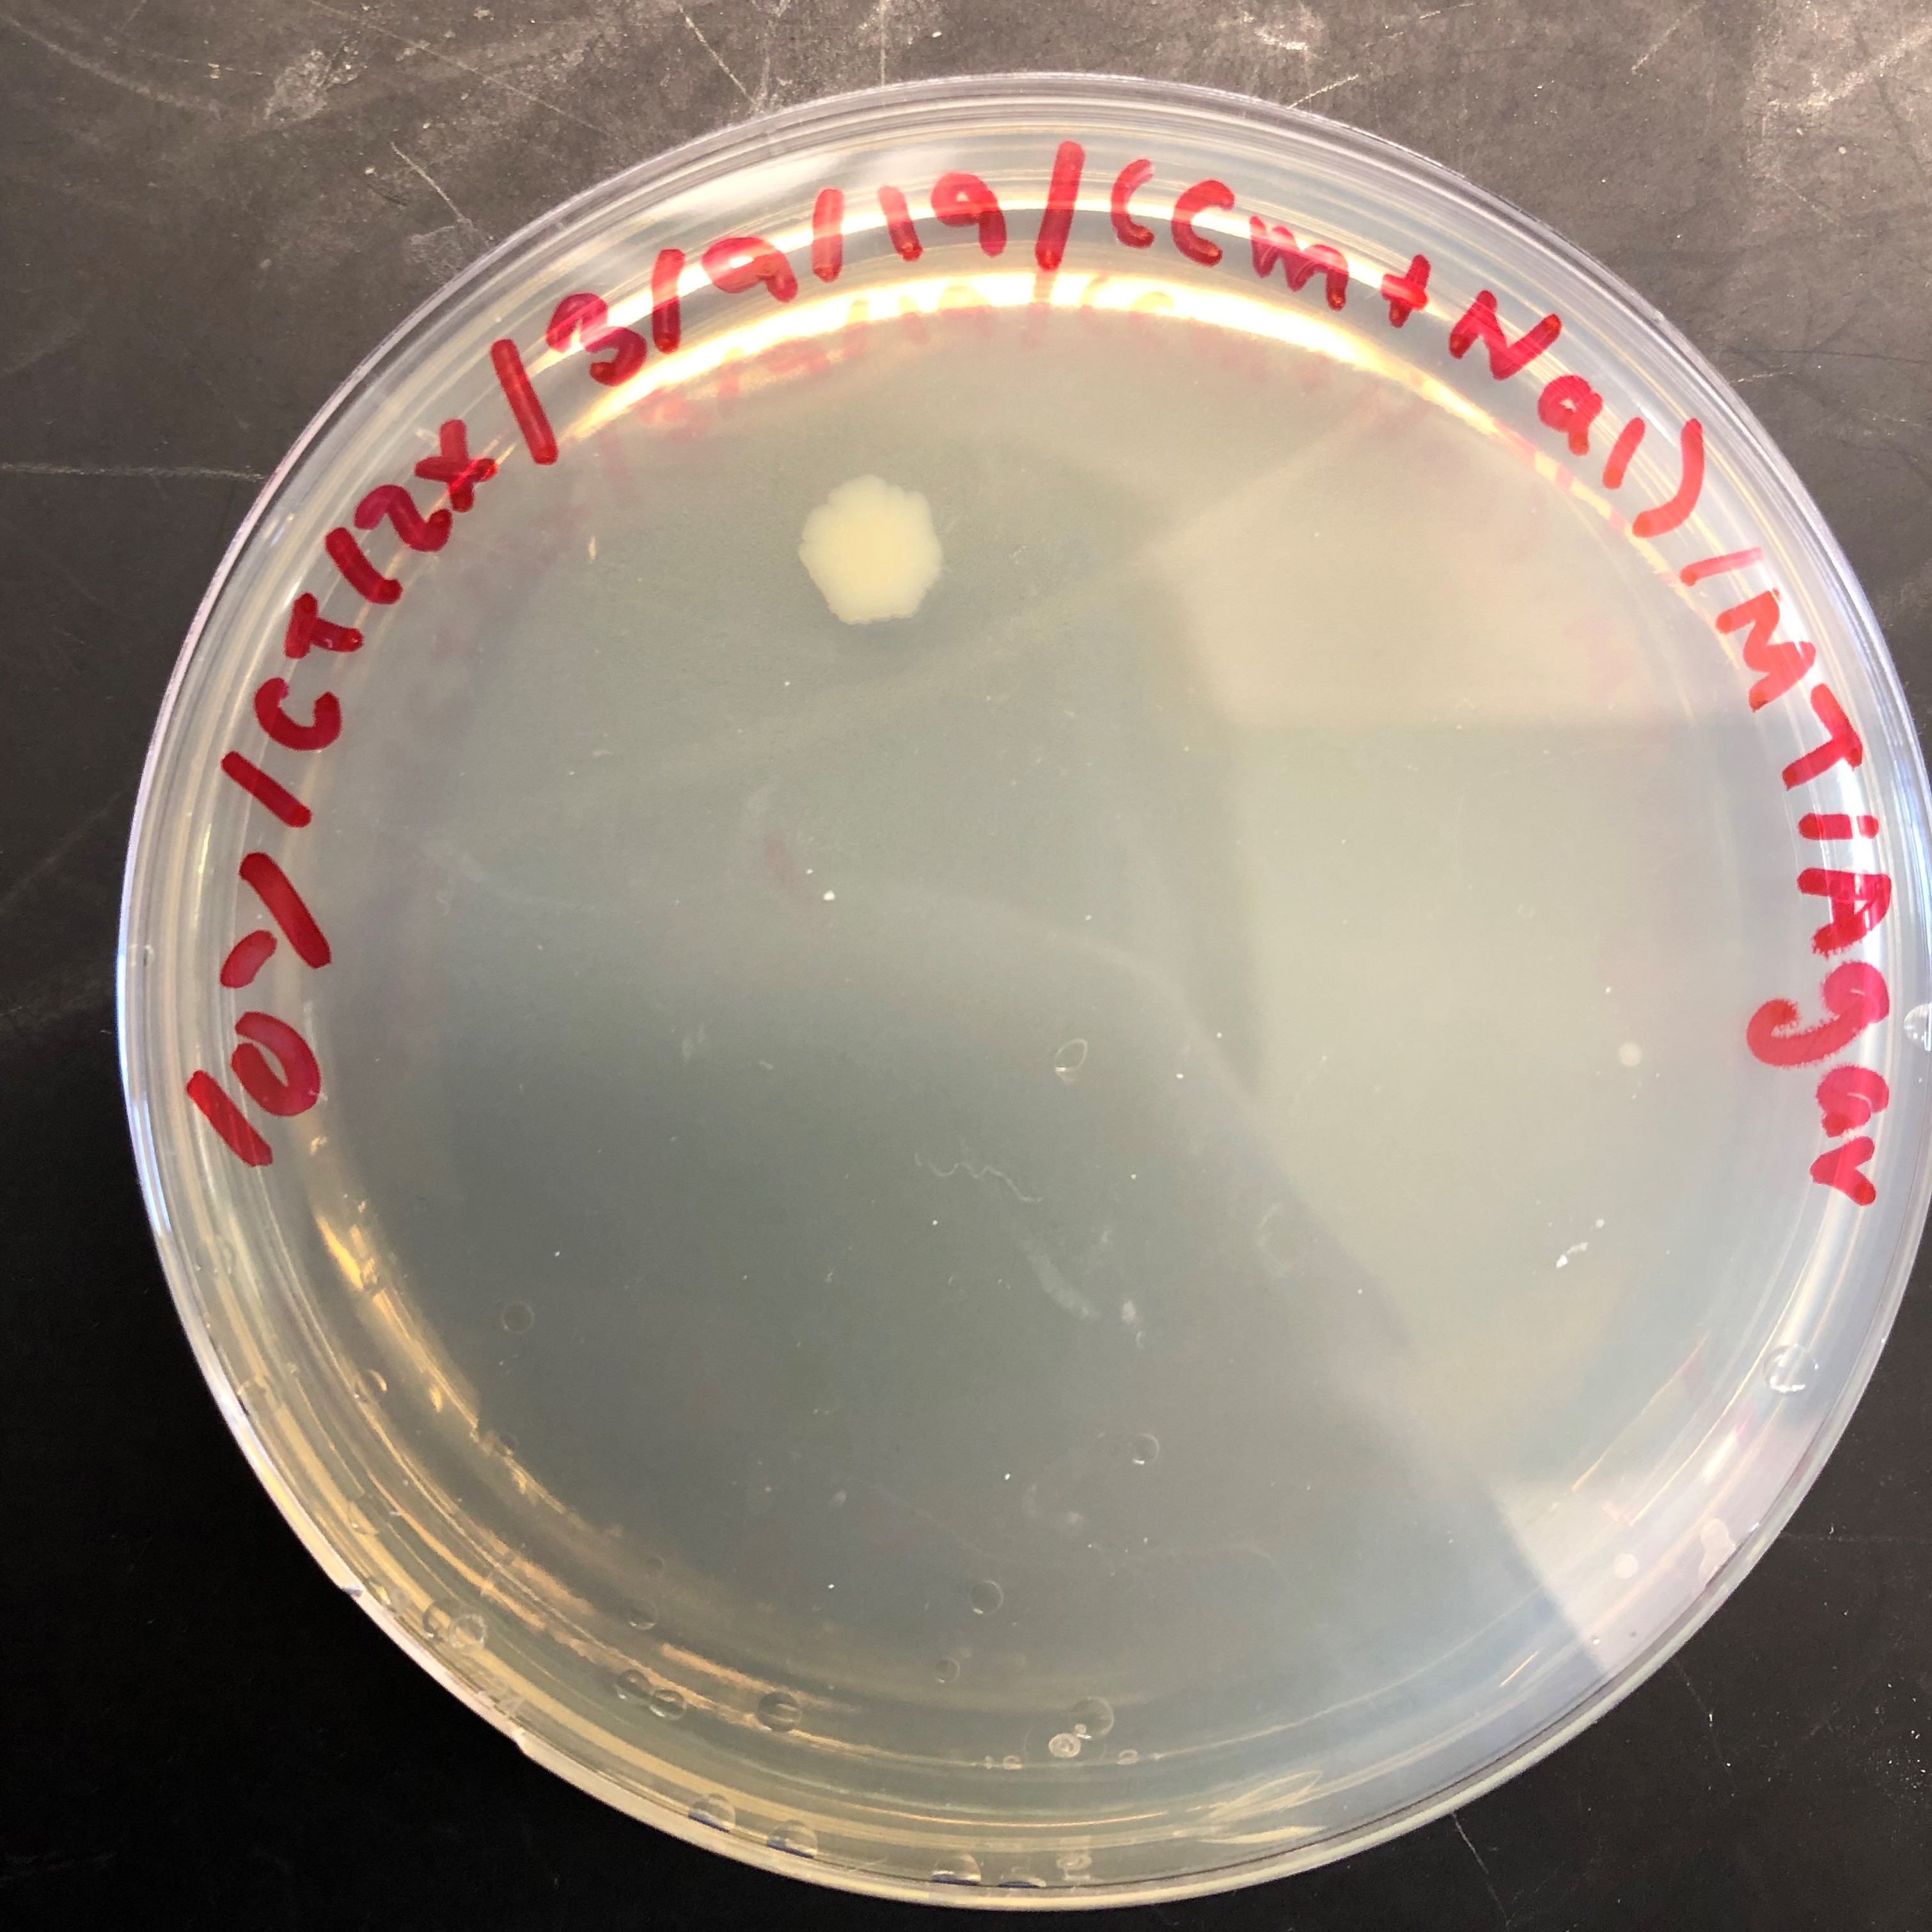
\includegraphics[width = 0.9\linewidth]{Mate_1_NalCm.jpg}
					\caption{MT $10^{-1} = 2$}
				\end{minipage}
				\begin{minipage}[t]{0.24\textwidth}
					\centering
					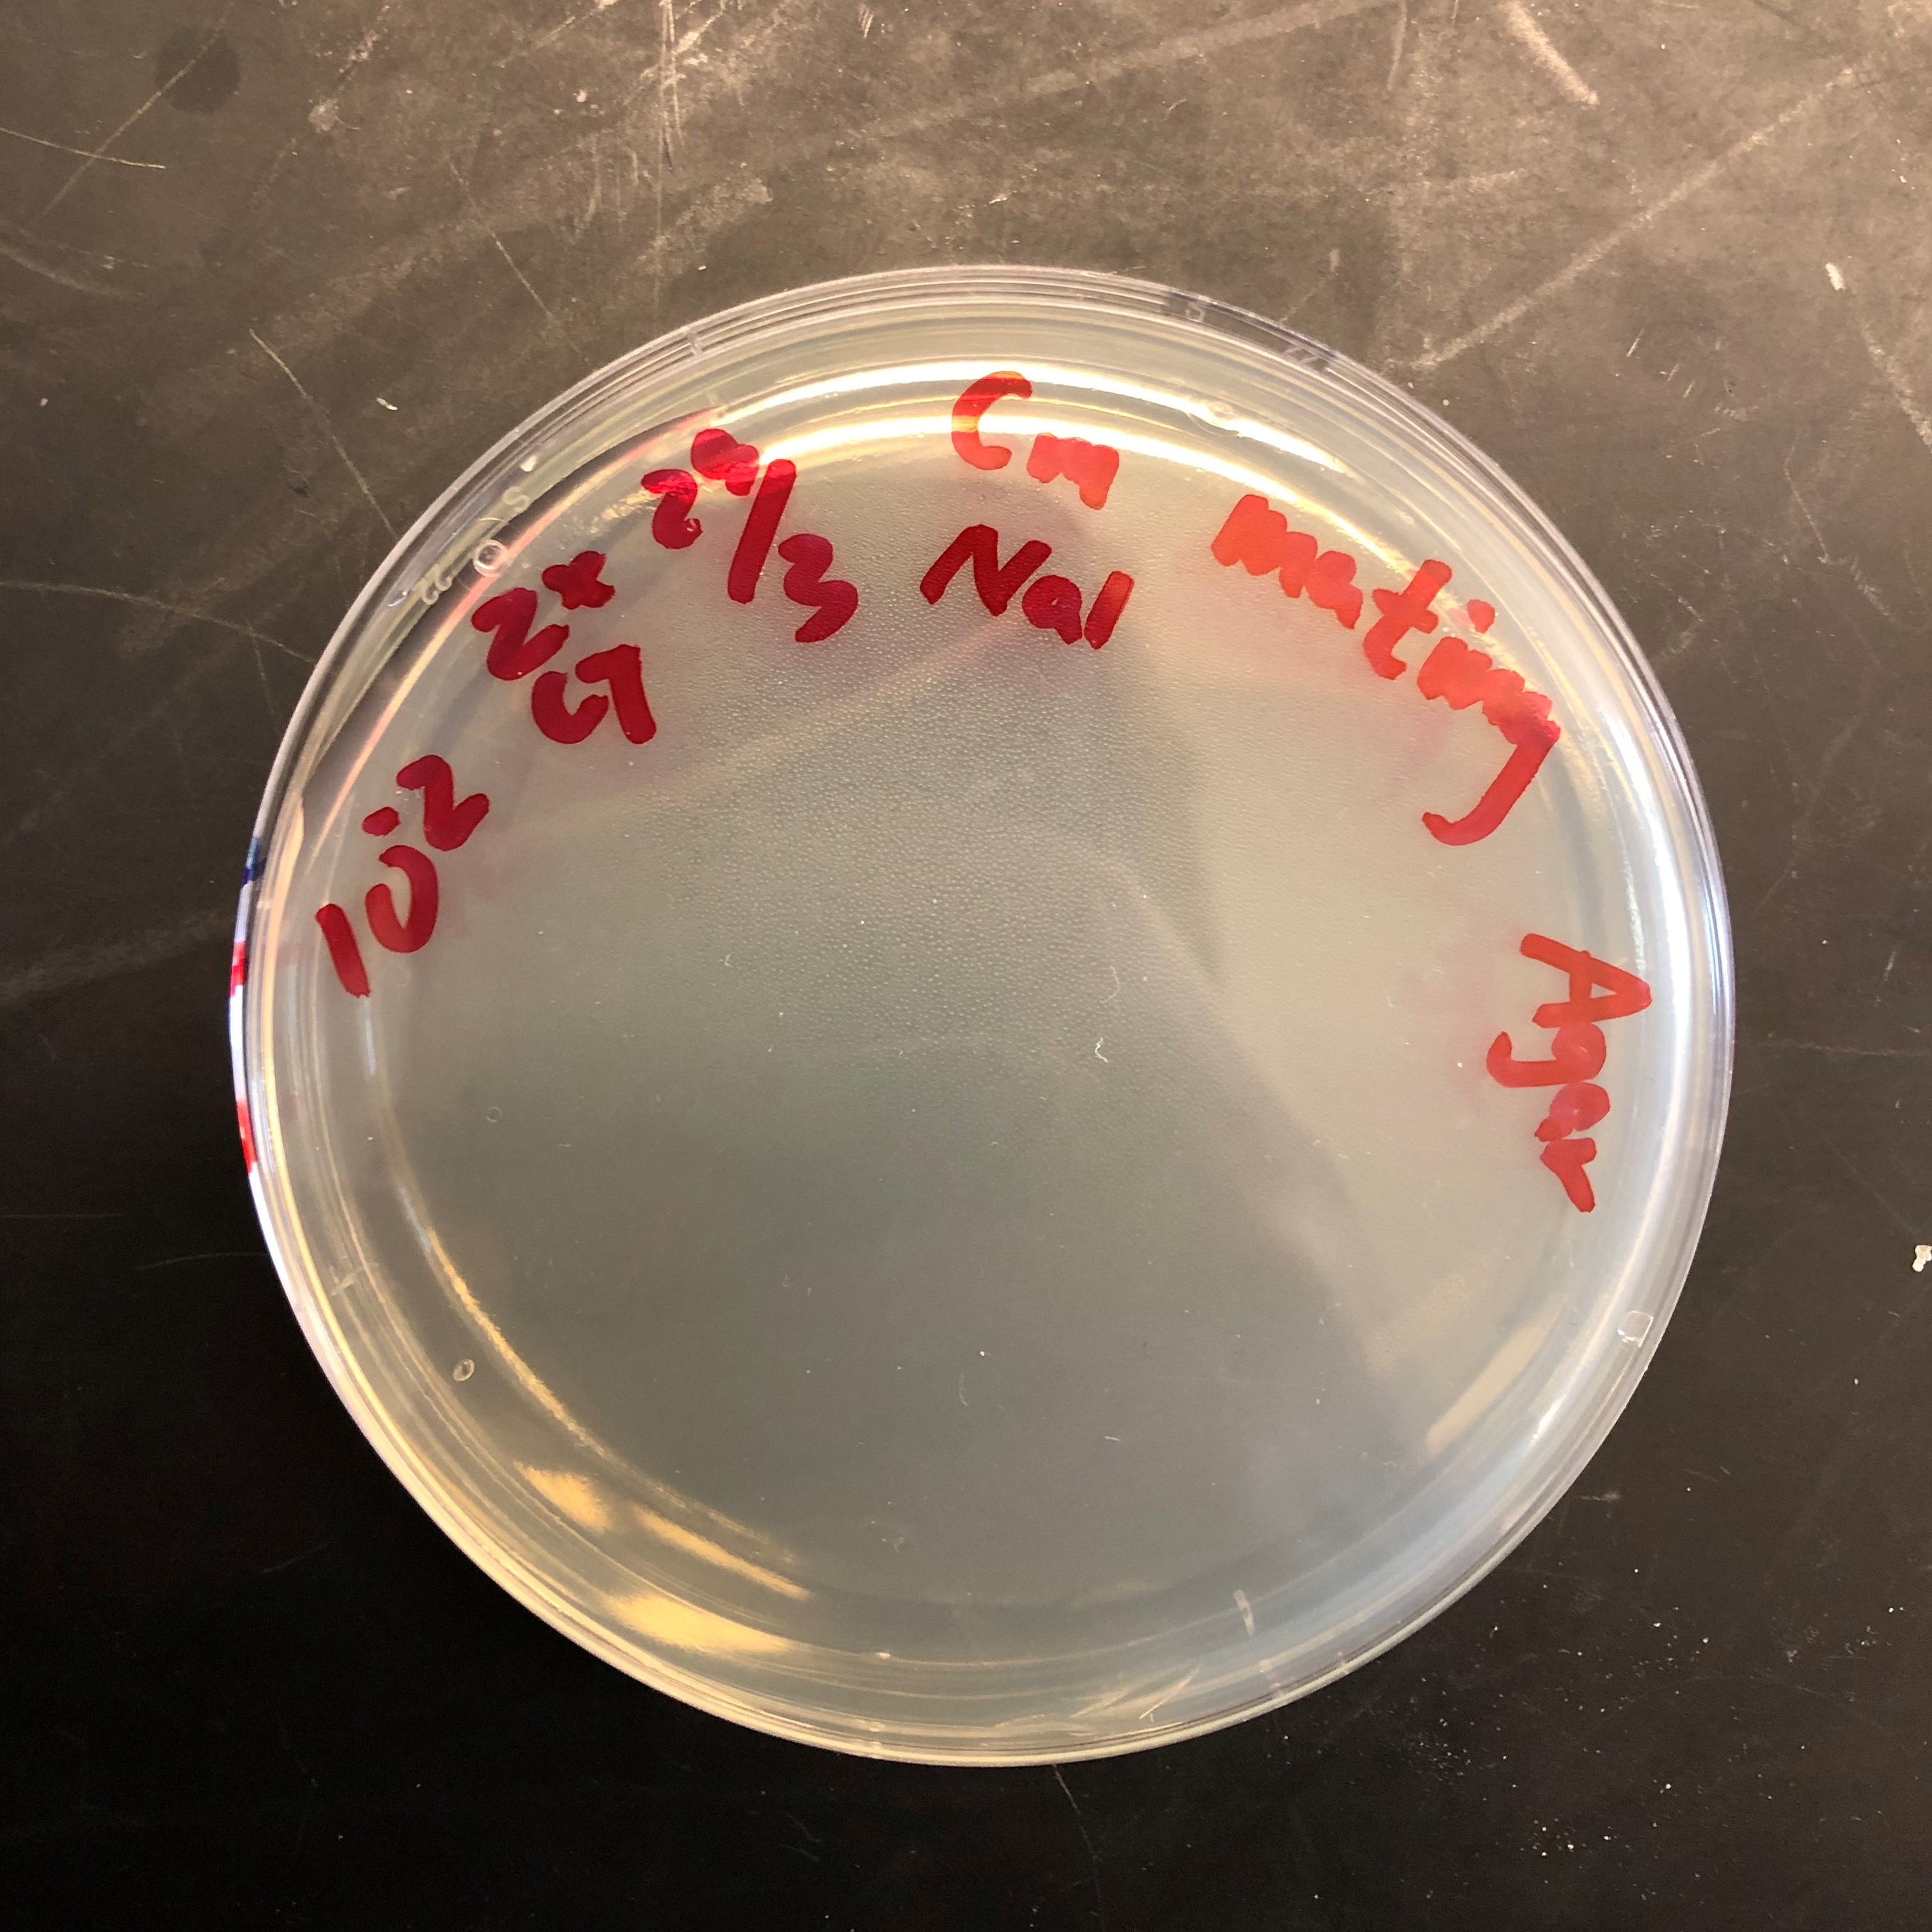
\includegraphics[width = 0.9\linewidth]{Mate_2_NalCm.jpg}
					\caption{MT $10 ^ {-2} = 0$}
				\end{minipage}
				\begin{minipage}[t]{0.24\textwidth}
					\centering
					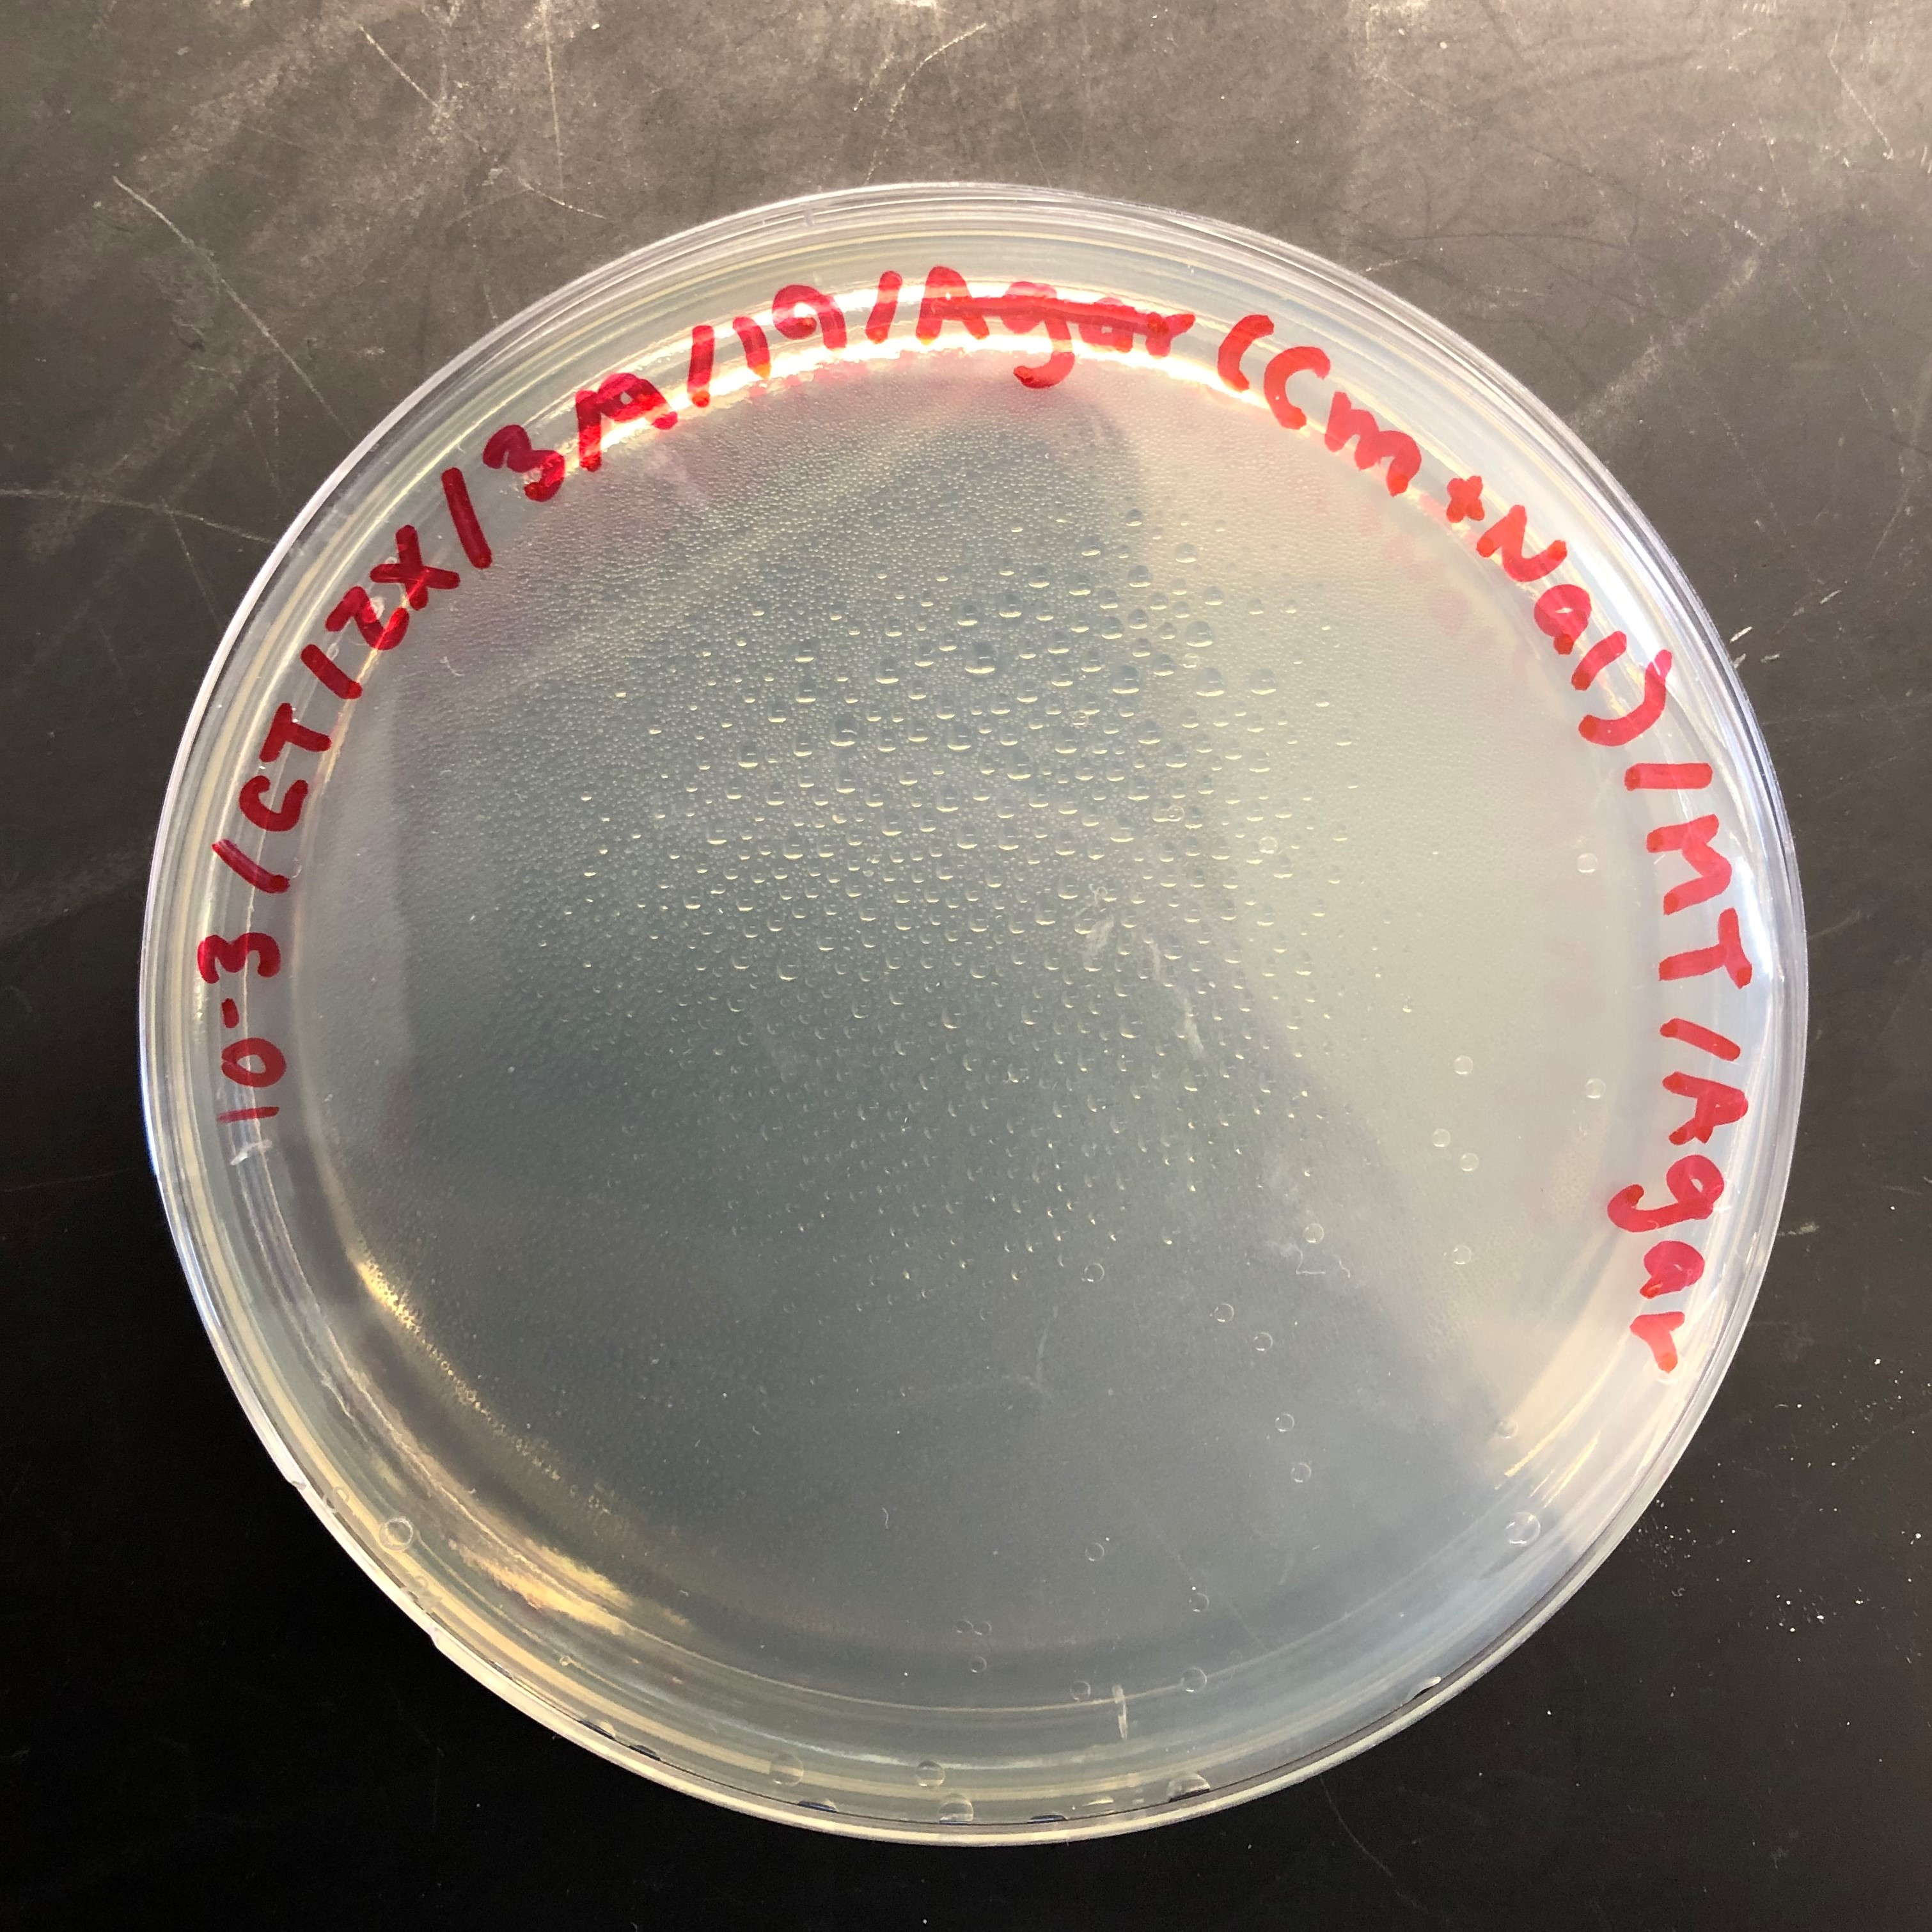
\includegraphics[width = 0.9\linewidth]{Mate_3_NalCm.jpg}
					\caption{MT $10 ^ {-3} = 0$}
				\end{minipage}
			\end{figure}
			\begin{figure}[H]
				\begin{minipage}[t]{0.32\textwidth}
					\centering
					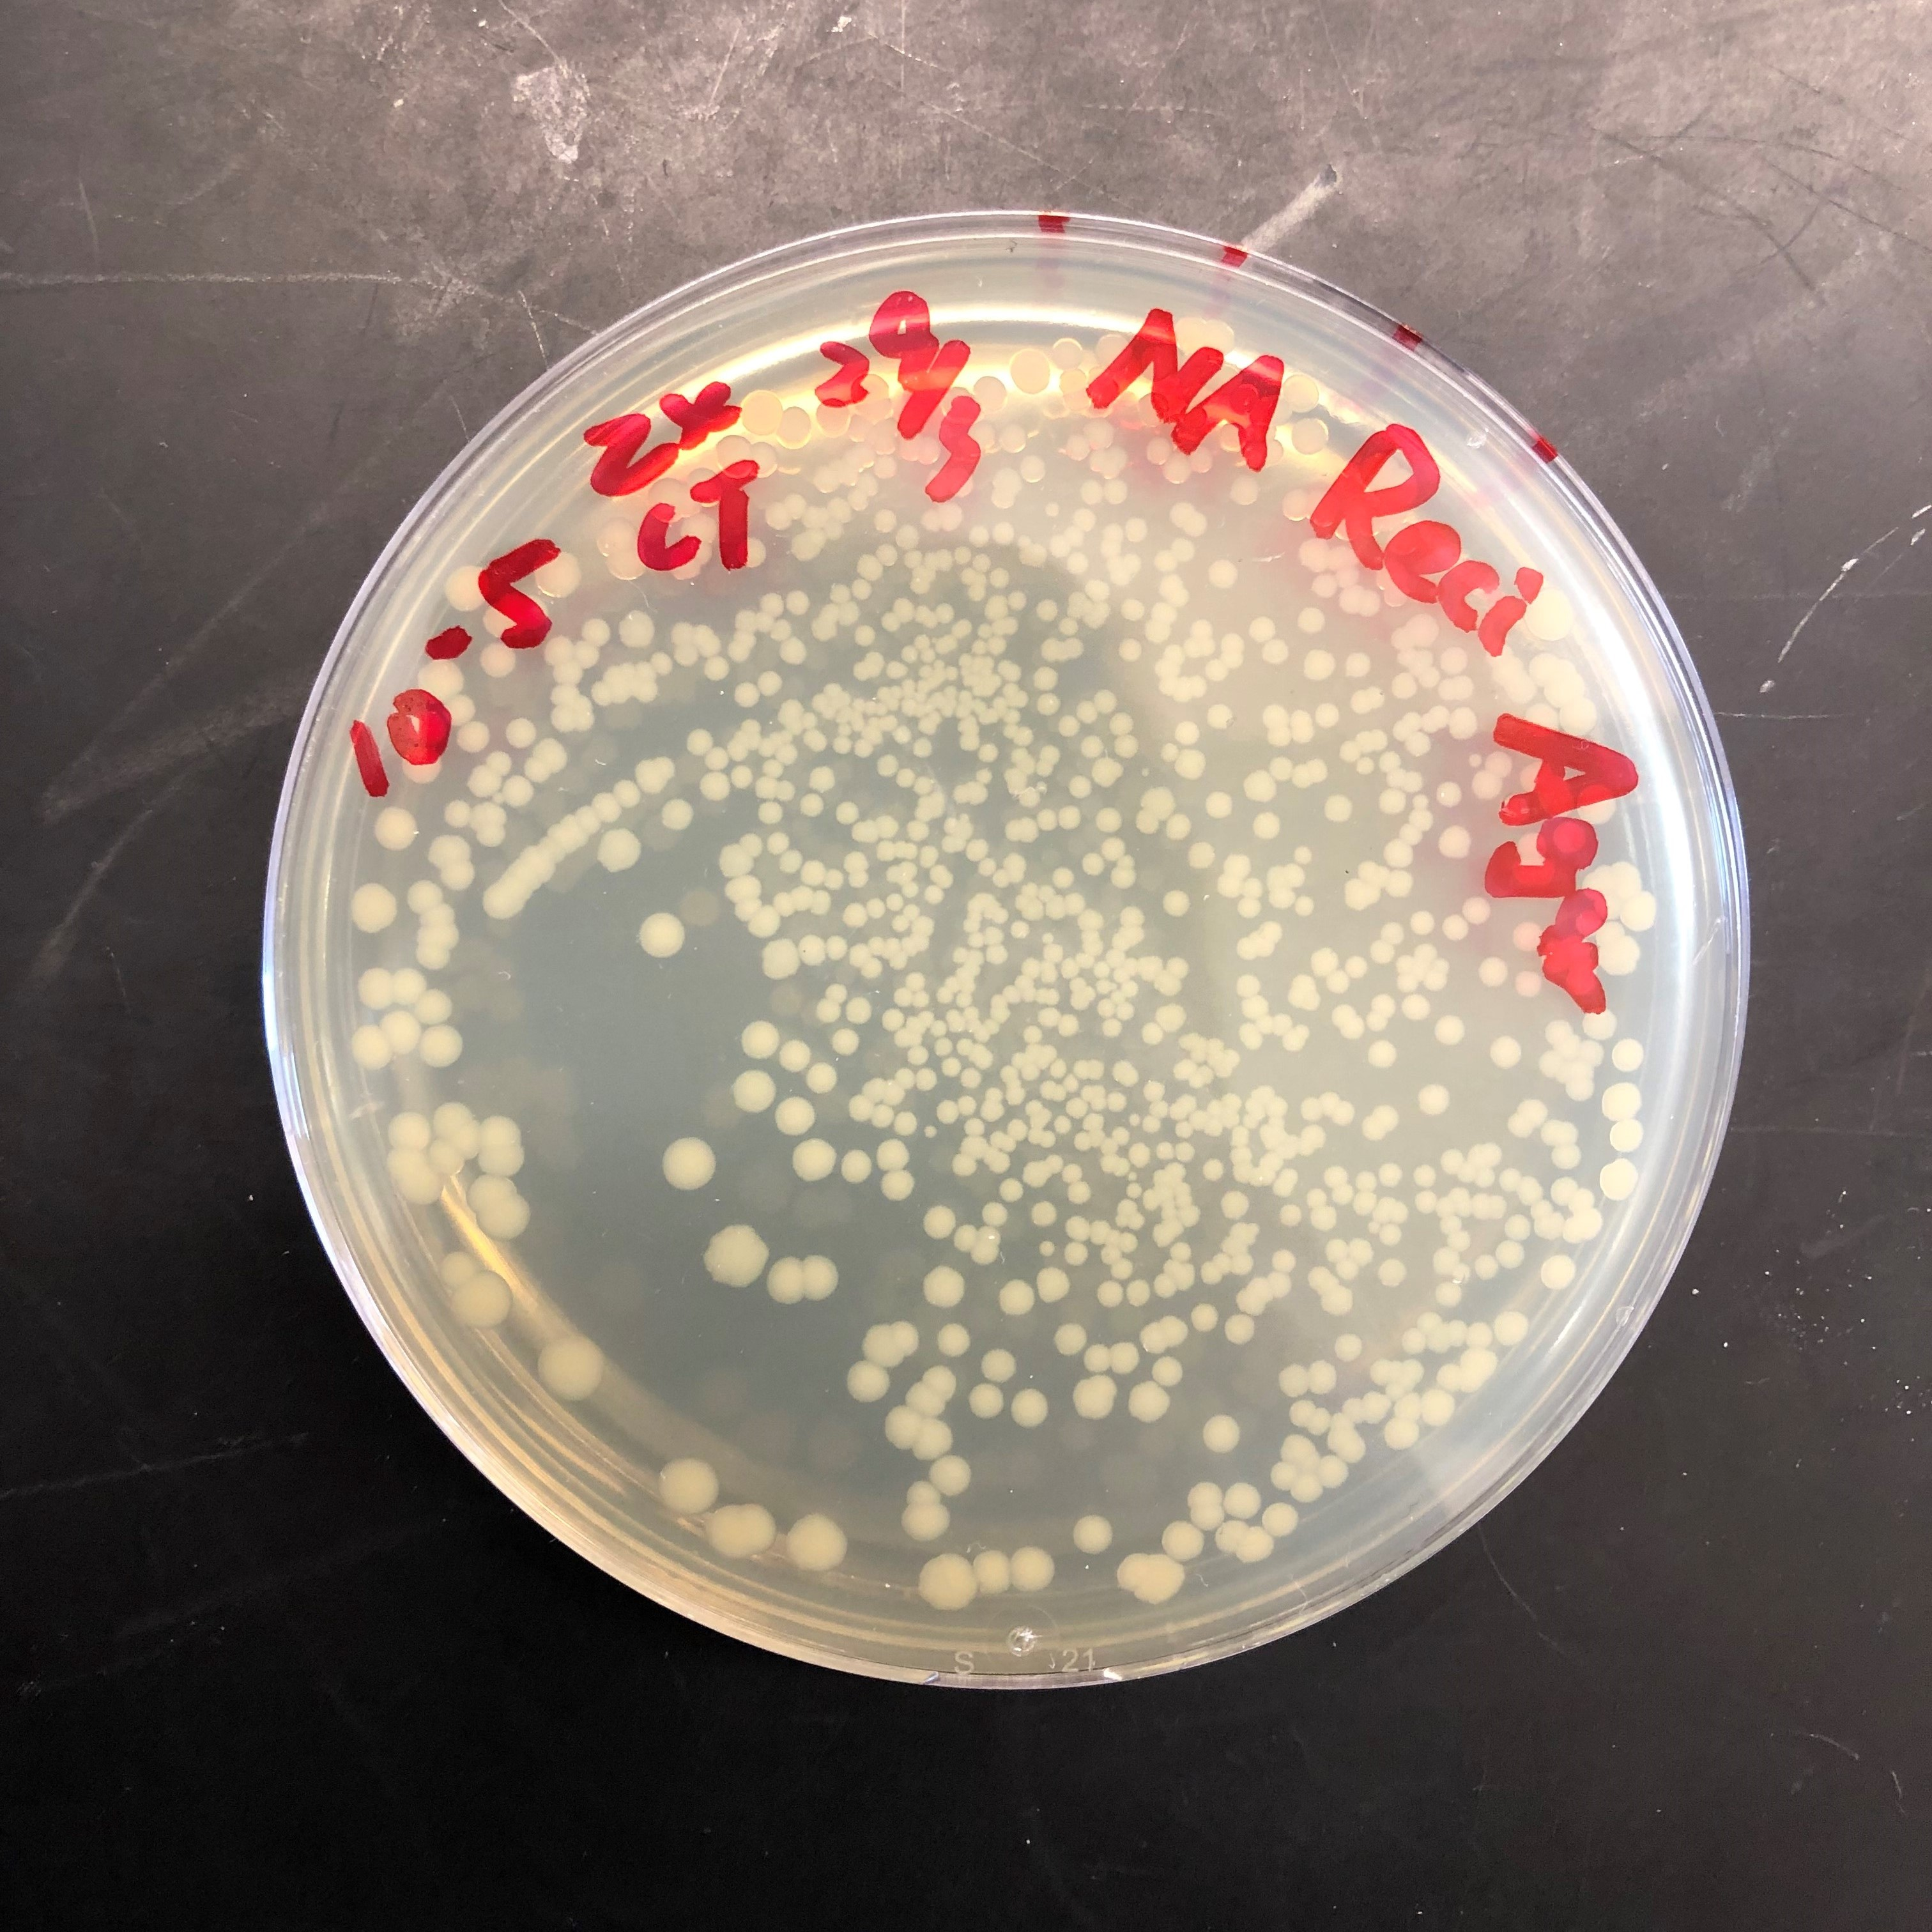
\includegraphics[width = 0.675\linewidth]{Reci_5_NA.jpg}
					\caption{R $10 ^ {-5} = 946$}
				\end{minipage}
				\begin{minipage}[t]{0.32\textwidth}
					\centering
					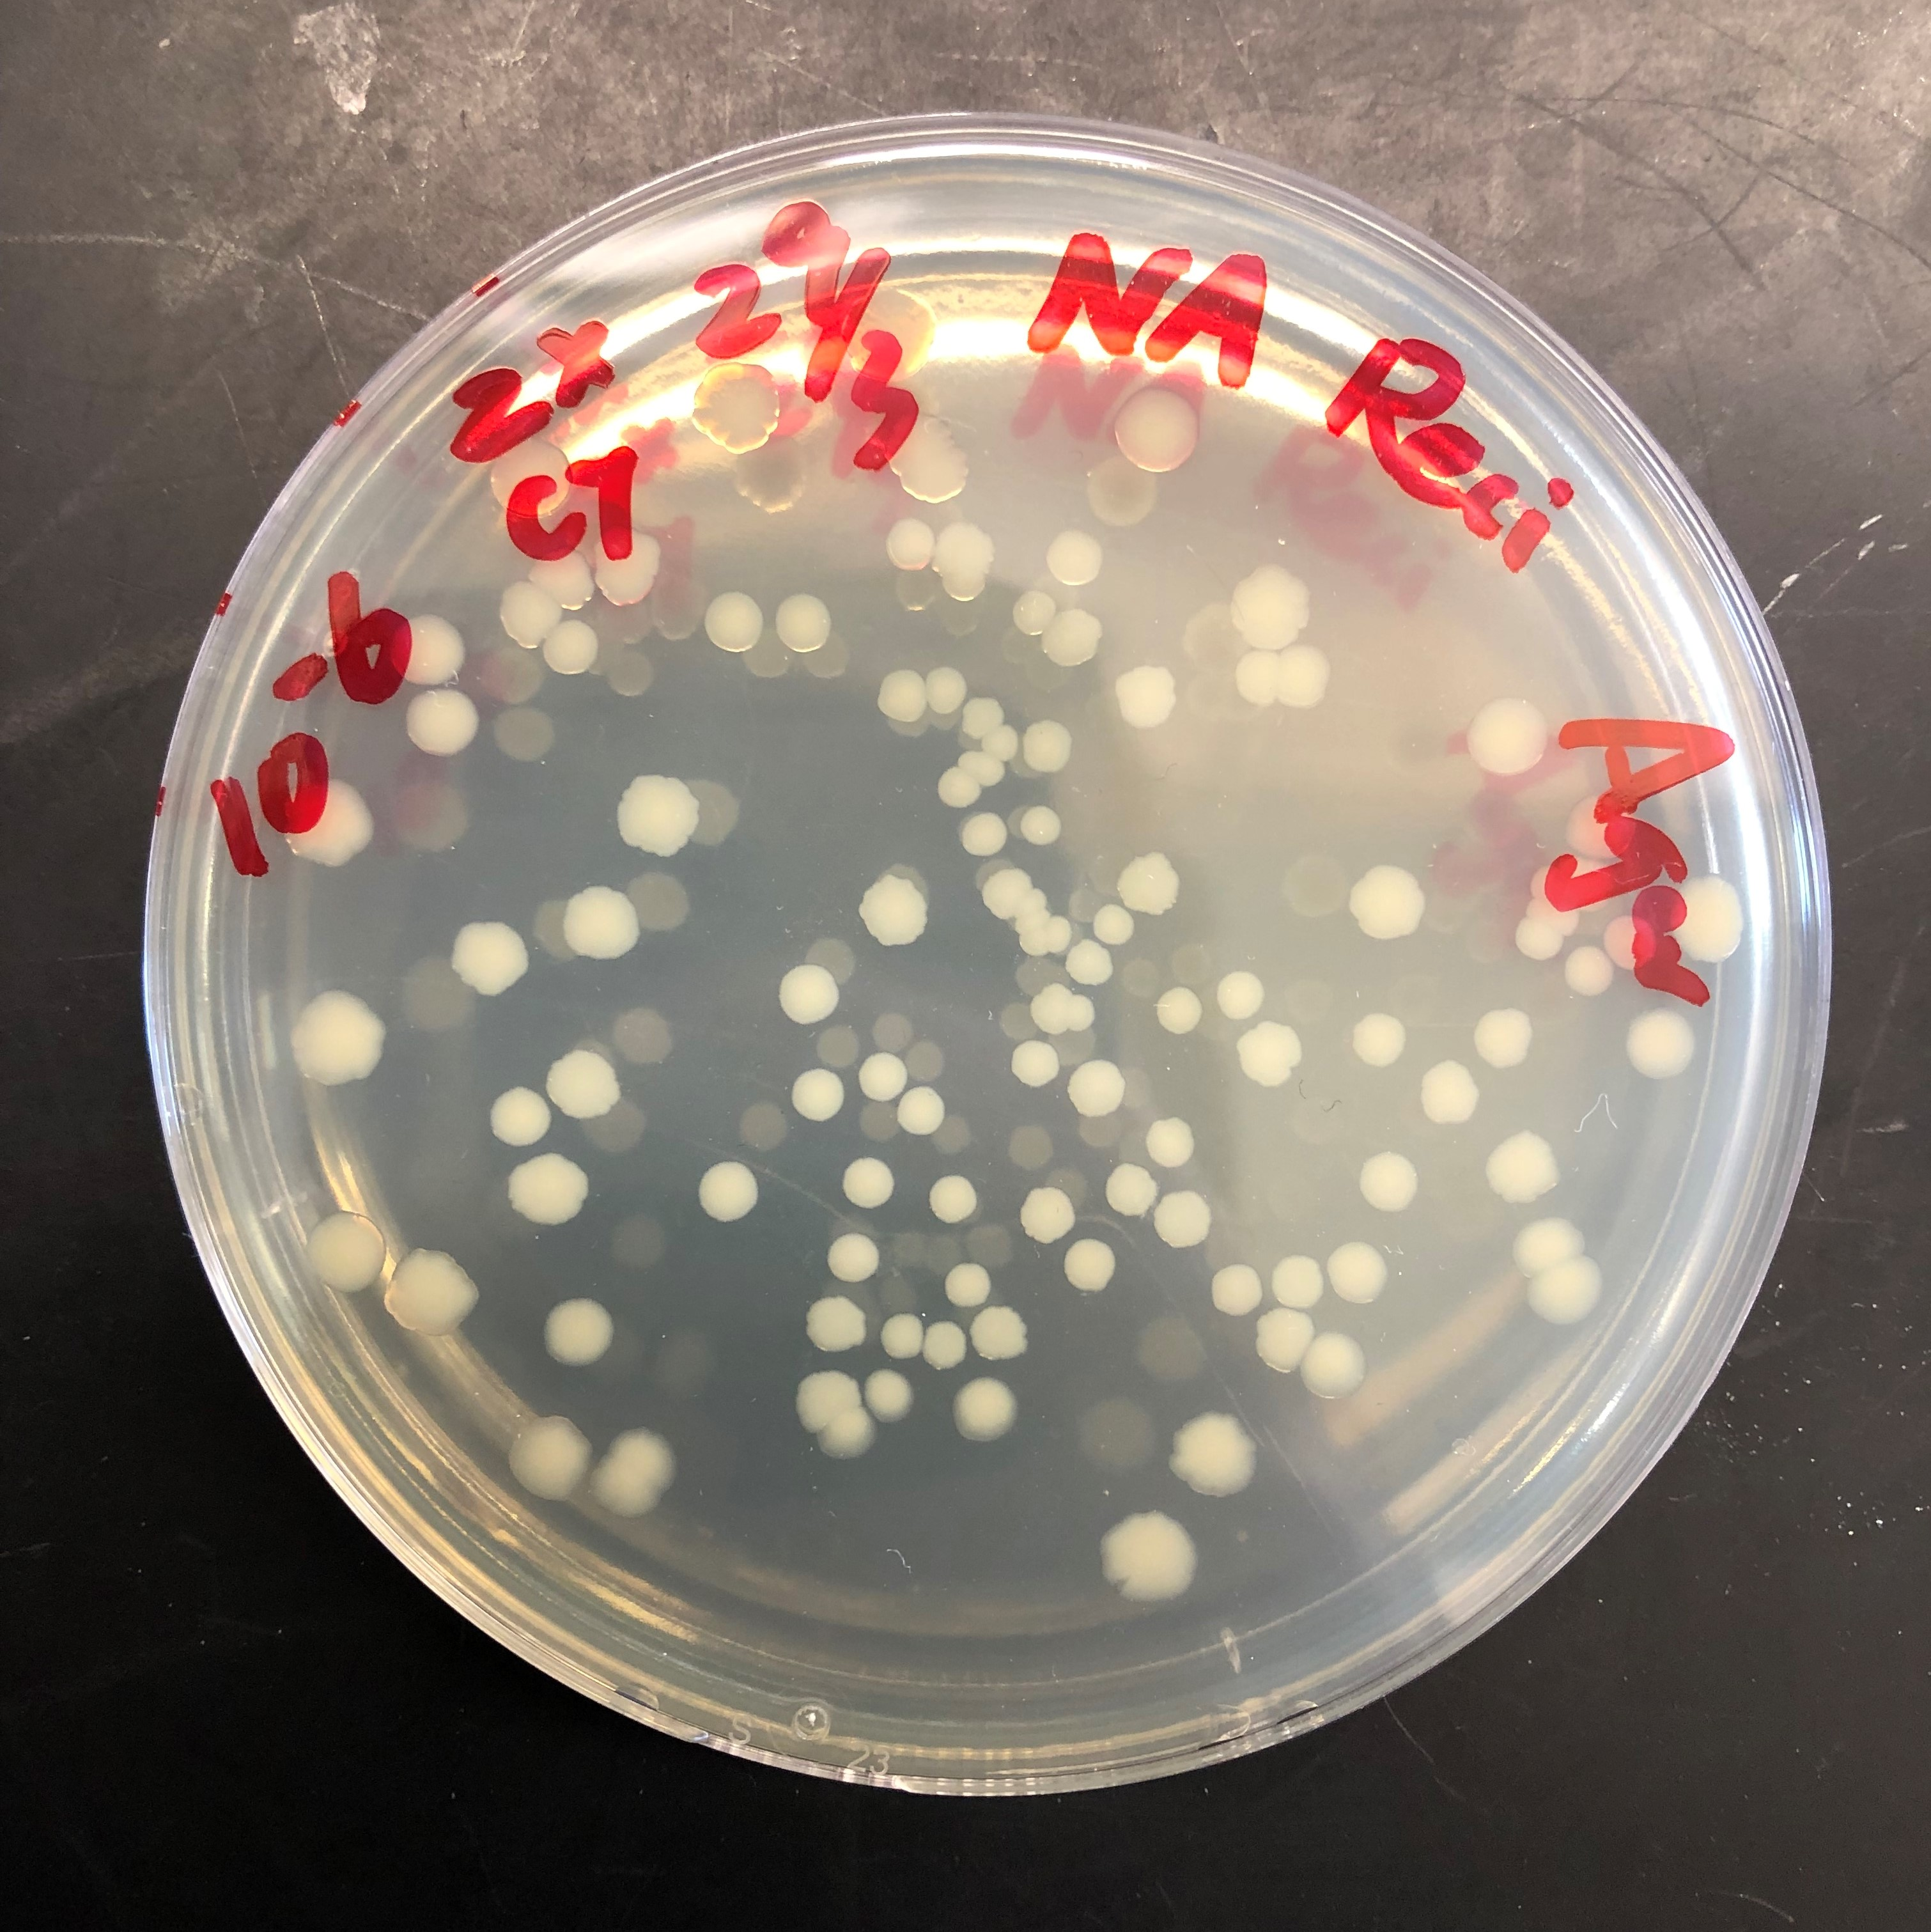
\includegraphics[width = 0.675\linewidth]{Reci_6_NA.jpg}
					\caption{R $10 ^{-6} = 107$}
				\end{minipage}
				\begin{minipage}[t]{0.32\textwidth}
					\centering
					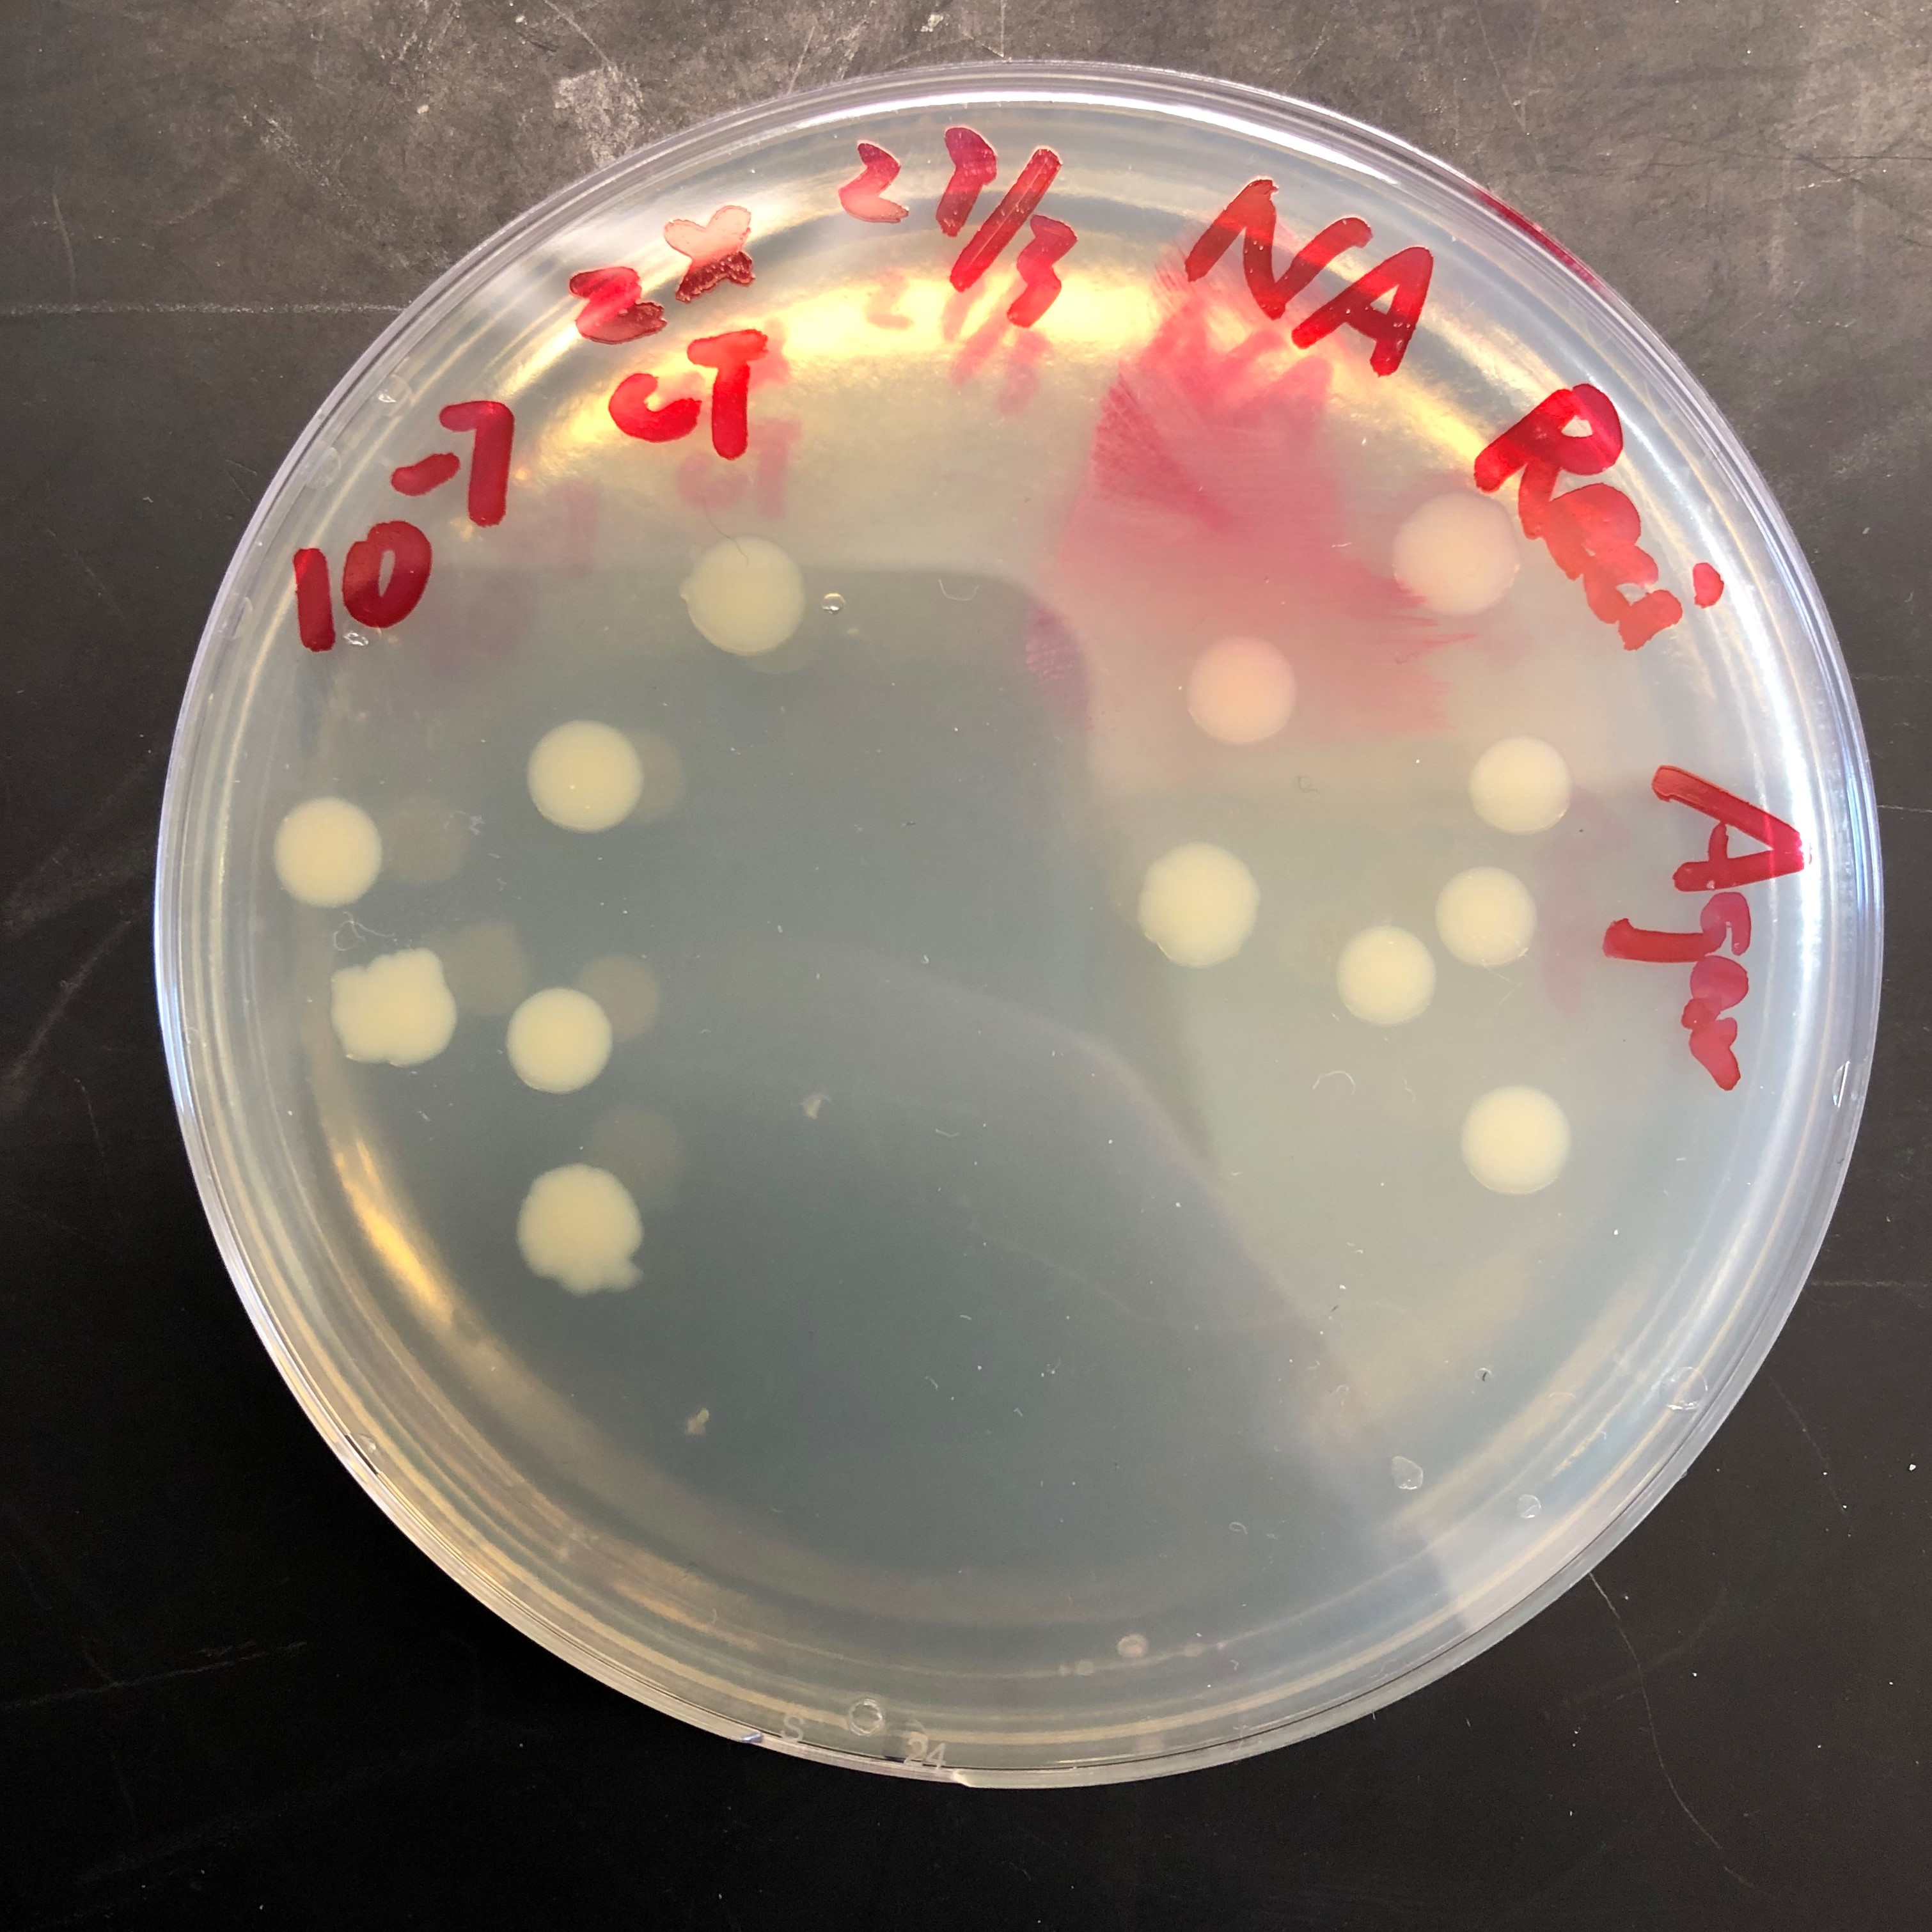
\includegraphics[width = 0.675\linewidth]{Reci_7_NA.jpg}
					\caption{R $10^{-7} = 13$}
				\end{minipage}
			\end{figure}
			\begin{figure}[H]
				\begin{minipage}[t]{0.5\textwidth}
					\centering
					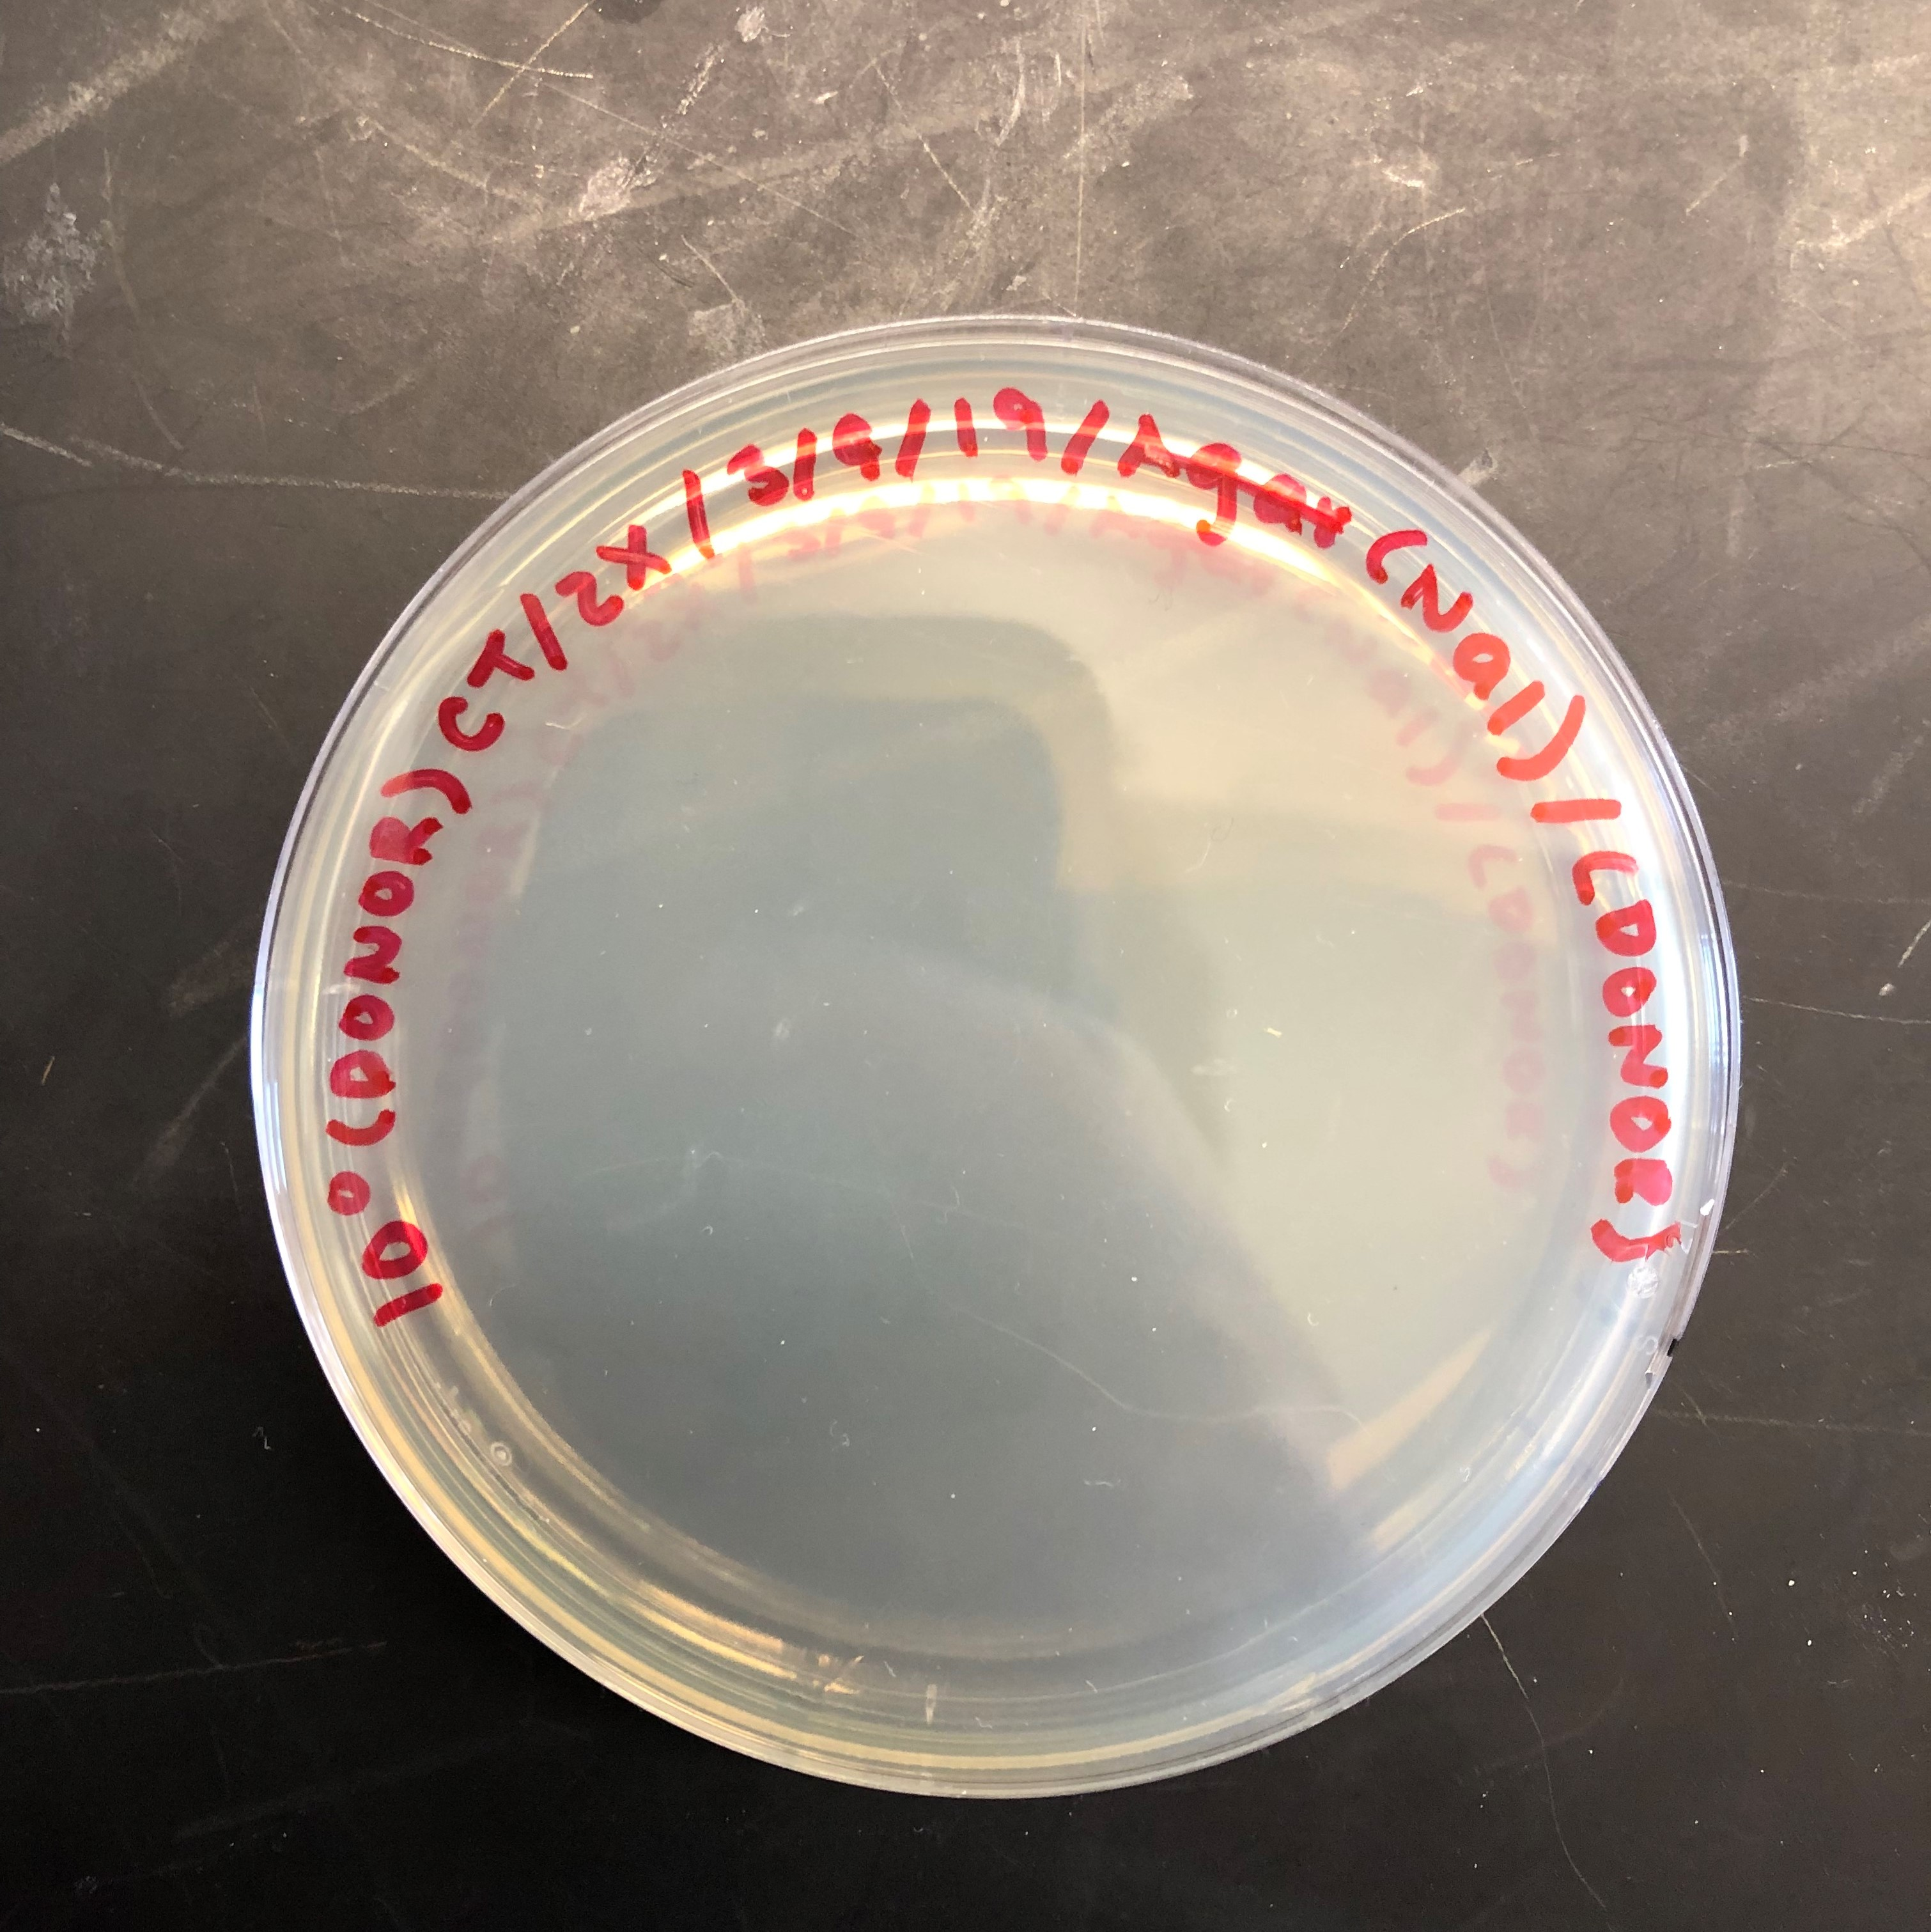
\includegraphics[width = 0.432\linewidth]{Done_0_Nal.jpg}
					\caption{D $10^0 = 0$}
				\end{minipage}
			\end{figure}
			\paragraph{General Description} The colonies are white and round. The size of colonies varies at the plates with $10 ^ 0$ dilution. This phenomenon indicates that if the plate starts with higher concentration of cells, the colonies are more likely to start from several cells instead of one single cell, which makes the size of colonies different.

			\paragraph{Percent Conjugation Calculation} 
\end{document}
